\documentclass[12pt,a4paper]{article}
\usepackage{cmap}
\usepackage{mathtext}
\usepackage{amsmath}
\usepackage{amsfonts}
\usepackage[T2A]{fontenc}
\usepackage[utf8]{inputenc} 
\usepackage[russian]{babel}
\usepackage[final]{graphicx}
\usepackage{multicol}
\usepackage{listings}
\usepackage{minted}
\usepackage{verbatim}
\usepackage{caption}
\usepackage{tabularx}
\usepackage[left=2cm, right=2cm, top=2cm, bottom=2cm]{geometry}
\graphicspath{}
\usepackage[unicode, pdftex]{hyperref}
\usepackage{float}
\DeclareGraphicsExtensions{.pdf,.png,.jpg}
    \usepackage{fancyhdr} % пакет для установки колонтитулов
    \pagestyle{fancy} % смена стиля оформления страниц
    \fancyhf{} % очистка текущих значений
    \fancyhead[C]{\thepage} % установка верхнего колонтитула
    \renewcommand{\headrulewidth}{0pt} % убрать разделительную линию

\hypersetup{colorlinks,
allcolors=[RGB]{010 090 200}} %красивые гиперссылки (не красные)
 
  %\makeatletter
%\renewcommand\section{\@startsection {section}{1}{\z@}%
 %     {-3.5ex \@plus -1ex \@minus -.2ex}%
  %    {2.3ex \@plus.2ex}%
   %  {\normalfont\Large\SS@sectfont}}
      
%\renewcommand\subsection{\@startsection{subsection}{2}{\z@}%
 %     {-3.25ex\@plus -1ex \@minus -.2ex}%
  %    {1.5ex \@plus .2ex}%
   %   {\normalfont\large\SS@subsectfont}}
\makeatother  
  \setcounter{secnumdepth}{4}
  \setcounter{tocdepth}{4}
\begin{document}
\def\contentsname{ОГЛАВЛЕНИЕ}
\thispagestyle{empty}
\begin{center}
\vspace{0.3cm}
\normalsize
{ФЕДЕРАЛЬНОЕ ГОСУДАРСТВЕННОЕ АВТОНОМНОЕ ОБРАЗОВАТЕЛЬНОЕ УЧРЕЖДЕНИЕ ВЫСШЕГО ОБРАЗОВАНИЯ} \par
%\vspace{0.3cm}
    \textbf{\guillemotleftСАНКТ-ПЕТЕРБУРГСКИЙ ПОЛИТЕХНИЧЕСКИЙ}
    \textbf{УНИВЕРСИТЕТ ПЕТРА ВЕЛИКОГО\guillemotright} \par
   % \vspace{0.3cm}
    {Институт Компьютерных наук и технологий}\par
    {Высшая школа искусственного интеллекта}\par
    {Направление 02.03.01 Математика и Компьютерные науки}
\end{center}
\vspace{-0.6cm}
\hrulefill
\vspace{-0.4cm}
\begin{center}
   \textcolor{gray}{\footnotesize{наименование организации - разработчика ТЗ на АС}}
\end{center}
\vfill
\begin{center}
    УТВЕРЖДАЮ \hspace{5.5cm} УТВЕРЖДАЮ
\end{center}
\begin{flushleft}
Руководитель \hspace{6.2cm} Разработчик (студент группы\newline
\phantom{Руководитель} \hspace{6.2cm} 5130201/20102) \vspace{0.2cm}\newline 
Курочкин Михаил Александрович \hspace{2.26cm} Гаар Владислав Сергеевич \vspace{0.2cm}\newline
\rule[0pt]{4cm}{0.5pt} \hspace{4.8cm} \rule[0pt]{4cm}{0.5pt} \vspace{-0.1cm} \newline
\begin{small}Личная подпись\end{small} \hspace{5.9cm} \begin{small}Личная подпись\end{small} \vspace{0.2cm}\newline
\rule[0pt]{4cm}{0.5pt} \hspace{4.8cm} \rule[0pt]{4cm}{0.5pt} \vspace{-0.1cm} \newline
\begin{small}Расшифровка подписи\end{small} \hspace{4.8cm} \begin{small}Расшифровка подписи\end{small} \vspace{0.2cm}\newline
Печать \hspace{7.43cm} Печать \vspace{0.1cm}\newline
Дата \hspace{7.85cm} Дата 
\end{flushleft}
\vspace{0.2cm}
\begin{center}
\large{Модуль кодирования и декодирования графа кодом Прюфера}
\end{center}
\vspace{-0.6cm}
\hrulefill
\begin{center}
\vspace{-0.4cm}
   \textcolor{gray}{\footnotesize{наименование вида АС}}
\end{center}
\vspace{0.4cm}
\begin{center}
\large{Процесс кодирования и декодирования графа кодом Прюфера}
\end{center}
\vspace{-0.6cm}
\hrulefill
\begin{center}
\vspace{-0.4cm}
   \textcolor{gray}{\footnotesize{наименование объекта автоматизации}}
\end{center}
\vspace{0.4cm}
\begin{center}
\large{Приложение}
\end{center}
\vspace{-0.6cm}
\hrulefill
\begin{center}
\vspace{-0.4cm}
   \textcolor{gray}{\footnotesize{сокращенное наименование АС}}
   \\
   \vspace{0.8cm}
\Large{\textbf{ТЕХНИЧЕСКОЕ ЗАДАНИЕ}}\\
\vspace{0.6cm}
\normalsize
На \rule[0pt]{2cm}{0.5pt} листах\\
\vspace{0.3cm}
Действует с \guillemotleft \rule[0pt]{0.8cm}{0.5pt}\guillemotright \rule[0pt]{2cm}{0.5pt} 20\rule[0pt]{0.5cm}{0.5pt} г.
\end{center}
\vspace{0.8cm}
СОГЛАСОВАНО\vspace{0.3cm}\newline
 Руководитель \vspace{0.3cm}\newline
 Курочкин Михаил Александрович\vspace{0.3cm}\newline
 \rule[0pt]{4cm}{0.5pt} \newline
 \begin{small}Личная подпись\end{small} \newline
 \rule[0pt]{4cm}{0.5pt} \newline
 \begin{small}Расшифровка подписи\end{small} \vspace{0.1cm}\newline
Печать\vspace{0.3cm}\newline
Дата 
\newpage
\tableofcontents
\newpage
\section{ОБЩИЕ ПОЛОЖЕНИЯ}
\subsection{Полное наименование системы и ее условное обозначение}
Полное наименование системы: Модуль кодирования и декодирования графа кодом Прюфера.\newline
\medskip Краткое наименование системы: Приложение.

\subsection{Номер договора (контракта)}
Отсутствует.

\subsection{Наименования организации-заказчика и организаций-участников работ}
Заказчик: Федеральное государственное автономное образовательное учреждение высшего образования <<Санкт-Петербургский политехнический университет Петра Великого>>. \\
Адрес заказчика: 195251 г. Санкт-Петербург, ул. Политехническая 29, корпус 4.
\newline
\newline
Разработчик: студент политехнического университета Петра Великого, гр. 5130201/20102, Гаар Владислав Сергеевич. \\
Адрес разработчика: 195220 г. Санкт-Петербург, ул. Гжатская 22, корпус 2. \\
Телефон: +79121738386\\
E-mail: gaarvlad@gmail.com

\subsection{Перечень документов, на основании которых создается система}
Отсутствует.

\subsection{Плановые сроки начала и окончания работы по созданию системы}\label{time}
Плановый срок начала работ по созданию Приложения \, --- 1 апреля 2024.  \\
Плановый срок окончания работ по созданию Приложения \, --- 20 мая 2024. 

\subsection{Источники и порядок финансирования работ}
Инициативная работа. Финансирование отсутствует.

\subsection{Порядок оформления и предъявления заказчику результатов работ по созданию системы}
При предъявлении результатов работ по созданию Приложения Заказчику передаётся персональный компьютер базовой 
комплектации, находящийся на гарантийном обслуживании, с установленной лицензионной ОС <<Windows 10>>, 
загрузочный модуль Приложения, руководство оператора, USB-носитель с копией Приложения, набор тестов.

\subsection{Перечень нормативно-технических документов, методических материалов, использованных при разработке ТЗ}
ГОСТ 34.602-89 <<Информационная технология. Комплекс стандартов на автоматизированные системы. Техническое задание
на создание автоматизированной системы>>.

\subsection{Определения, обозначения и сокращения}
ТЗ -- техническое задание. \medskip \newline
АС -- автоматизированная система. \medskip \newline
ОС -- операционная система.\medskip \newline
ПК -- персональный компьютер.

\newpage
\section{НАЗНАЧЕНИЕ И ЦЕЛИ СОЗДАНИЯ СИСТЕМЫ}
\subsection{Назначение системы}
Назначением системы является автоматизация процесса управления данными структуры графа в виде последовательности 
кодов Прюфера.

\subsection{Цели создания системы}
Целью создания системы является сокращение времени передачи информации о структуре графа за счёт использования 
кода Прюфера.

\newpage
\section{ХАРАКТЕРИСТИКА ОБЪЕКТА АВТОМАТИЗАЦИИ}
Объектом автоматизации является граф со следующими характеристиками:
\begin{itemize}
    \item взвешенный;
    \item связный;
    \item направленный;
    \item ациклический;
\end{itemize}

\begin{comment}
\noindent Автоматизируемая система должна обеспечивать следующие функции:
\begin{itemize}
    \item[--] генерация случайного взвешенного связного направленного ациклического графа,
    \item[--] кодирование графа в последовательность кодов Прюфера с учетом весов рёбер, 
    \item[--] декодирование последовательности кодов Прюфера для восстановления исходного графа с весами рёбер, 
    \item[--] валидация исходных данных на корректность, 
    \item[--] проверка корректности декодирования,
    \item[--] вывод полученного результата.
\end{itemize} 
\end{comment}

\medskip Приложение рассчитано на обработку графов с числом вершин от 1 до 1000 и поддерживает взвешенные рёбра, 
представленные числовыми значениями с точностью до двух знаков после запятой.

\newpage
\section{ТРЕБОВАНИЯ К СИСТЕМЕ}
\subsection{Требования к системе в целом}
\subsubsection{Требования к структуре и функционированию системы}
\paragraph{Перечень подсистем, их назначение и основные характеристики} \label{system}\mbox{}\medskip\\
\noindent Аппаратная часть состоит из персонального компьютера базовой комплектации, находящегося на гарантийном 
обслуживании. Требования к минимальной технической характеристике персонального компьютера для запуска Приложения:
\begin{itemize}
    \item Процессор с тактовой частотой 1,2 ГГц.
    \item Объем оперативной памяти 256 Мб.
    \item Жёсткий диск 80 Гб.
    \item Файловая система NTFS/FAT32/exFAT.
    \item Разъём USB 3.0.
\end{itemize}

\noindent Программная часть состоит из Приложения, лицензионной операционной системы \linebreak Windows 10, 
лицензионной среды разработки Microsoft Visual Studio 2022.

\paragraph{Требования к способам и средствам связи для информационного обмена между компонентами системы} \mbox{}\medskip\\
Требования не предъявляются.

\paragraph{Требования к характеристикам взаимосвязей создаваемой системы со смежными системами} \mbox{}\medskip\\
Требования не предъявляются.

\paragraph{Требования к режимам функционирования системы}\mbox{}\medskip\\
Приложение должно иметь активный режим функционирования и использоваться не более 10 часов в день, 7 дней в неделю.

\paragraph{Требования по диагностированию системы}\mbox{}\medskip\\
Требования не предъявляются.

\paragraph{Перспективы развития, модернизации системы}\mbox{}\medskip\\
Требования не предъявляются.

\subsubsection{Требования к численности и квалификации персонала системы}\label{412}
Рекомендуемая численность для эксплуатации Приложения: 1 человек. \\

\noindent Пользователь Приложения должен:
\begin{itemize}
    \item[--] иметь опыт работы с персональным компьютером на базе операционных систем Microsoft Windows на начальном уровне;
    \item[--] изучить руководство оператора, предоставленное Исполнителем.
\end{itemize}

\subsubsection{Показатели назначения}
Приложение должно обеспечивать следующие количественные показатели, которые характеризуют степень соответствия назначению:
\begin{itemize}
    \item[--] Время генерации взвешенного связного направленного ациклического графа не должно превышать 1 секунды
    при числе вершин до 1000.
    \item[--] Время выполнения кодирования графа не должно превышать 2 секунд при числе вершин до 1000.
    \item[--] Время выполнения декодирования кода Прюфера для восстановления графа не должно превышать 2 секунд 
    при числе вершин до 1000.
    \item[--] Время отклика пользовательского меню не должно превышать 0.1 секунду.
\end{itemize}

\subsubsection{Требования к надежности}
Надежность обеспечивается:
\begin{enumerate}
    \item аппаратным обеспечением, находящимся на гарантийном обслуживании;
    \item лицензионным программным обеспечиванием Microsoft Windows 10 и лицензионной средой разработки Microsoft 
    Visual Studio 2022;
    \item математически корректным обеспечением;
    \item соответствием процесса разработки Приложения ГОСТ Р ИСО/МЭК 25010-2015 <<Требования и оценка качества 
    систем и программного обеспечения>>.
\end{enumerate}

% Система должна сохранять работоспособность и обеспечивать восстановление своих функций при возникновении 
% следующих внештатных ситуаций:
% \begin{itemize}
%     \item[--] при сбоях в системе электроснабжения аппаратной части, приводящих к перезагрузке ОС, восстановление
%     программы должно происходить после перезапуска ОС и запуска исполняемого файла системы; 
%     \item[--] при ошибках в работе аппаратных средств (кроме носителей данных и программ) восстановление функции
%     системы возлагается на ОС; 
%     \item[--] при ошибках, связанных с программным обеспечением (ОС и драйверы устройств), восстановление 
%     работоспособности возлагается на ОС. Для защиты аппаратуры от бросков напряжения и коммутационных помех 
%     должны применяться сетевые фильтры.
% \end{itemize}


\subsubsection{Требования к безопасности}\label{safety}
Факторы, оказывающие вредные воздействия на здоровье со стороны всех элементов системы не должны превышать 
действующих норм СанПиН 2.2.2./2.4.1340-03 <<Гигиенические требования к персональным 
электронно-вычислительным машинам и организации работы>> (п. 10, п. 11). \medskip \newline
Рабочее помещение оператора Приложения должно соответствовать нормам СанПиН 2.2.4. 129403 <<2.2.4. Физические
факторы производственной среды. Гигиенические требования к аэроионному составу воздуха производственных и общественных
помещений>> (п. 3). \medskip \newline
Все внешние элементы технических средств системы, находящиеся под напряжением, должны соответствовать 
ГОСТ 12.1.030-81 <<Система стандартов безопасности труда>> (п. 7).

\subsubsection{Требования к эргономике и технической эстетике} \label{ergo}
\noindent Эксплуатация должна проходить в закрытых помещениях офисного типа, соответствующих ГОСТ 30494-2011
<<Параметры микроклимата в помещениях>> (п. 5). \medskip \newline
Рабочее место пользователя должно удобным, оборудовано столом и стулом, соответствовать ГОСТ Р 50923-96
<<Дисплеи. Рабочее место оператора. Общие эргономические требования в производственной среде. Методы измерения>>.
(п. 4, п. 5). \medskip \newline
Интерфейс должен быть рассчитан на преимущественное использование клавиатуры, то есть управление системой должно осуществляться с помощью текстовго ввода команд. 

\subsubsection{Требования к транспортабельности для подвижных АС}
Требования не предъявляются.

\subsubsection{Требования к эксплуатации, техническому обслуживанию, ремонту и хранению компонентов системы}
ПК должен находиться на гарантийном обслуживании.

\subsubsection{Требования к защите информации от несанкционированного доступа}
Требования не предъявляются.

\subsubsection{Требования по сохранности информации при авариях}\label{trouble}
Приложение должно храниться на жёстком диске ПК, ПК должен находиться на гарантийном обслуживании и быть
оснащён источником бесперебойного питания, обеспечивающим работу в течение 5 минут при перепадах напряжения. \medskip \newline
Копия Приложения должна храниться на USB-носителе в другом помещении, чтобы обеспечивать возможность повторной загрузки Приложения 
на ПК при авариях. Время восстановления модуля Приложения -- 20 секунд. \medskip \newline
Авариями считаются отключение электропитания, скачки напряжения, что ведёт к потере сессионных данных Приложения.

\subsubsection{Требования к защите от влияния внешних воздействий}
Рабочее помещение должно удовлетворять требованиям радиационной безопасности, изложенным в СанПиН 2.6.1.2800-10 
<<Требования радиационной  безопасности при облучении населения природными источниками ионизирующего излучения>> 
(п. 3.2, п. 4.2)

\subsubsection{Требования к патентной чистоте}
Требования не предъявляются.

\subsubsection{Требования по стандартизации и унификации}
Требования не предъявляются.

\subsubsection{Дополнительные требования}
Требования не предъявляются.

\subsection{Требования к функциям (задачам), выполняемым системой} \label{functions}
Исполнителю необходимо выполнить следующие задачи:
\begin{itemize} 
    \item[--] генерация случайного взвешенного связного направленного ациклического графа,
    \item[--] кодирование графа в последовательность кодов Прюфера с учетом весов рёбер, 
    \item[--] декодирование последовательности кодов Прюфера для восстановления исходного графа с весами рёбер, 
    \item[--] вывод полученного результата.
\end{itemize}

Для выполнения поставленных задач Исполнителю необходимо реализовать следующие функции:

\begin{itemize}
    \item функция выбора способа создания графа: ручной, случайный;
    \item функция ввода количества вершин пользователем;
    \item функция генерации случайного взвешенного связного направленного ациклического графа с введённым 
    количеством вершин;
    \item функция кодирования взвешенного связного направленного ациклического графа с использованием алгоритма
    построения кода Прюфера;
    \item функция декодирования последовательности кода Прюфера для восстановления исходного графа
    с рёбрами и их весами;
    \item функция вывода меню на экран;
    \item функция контроля входных данных;
    \item функция вывода полученного результата.
\end{itemize}


\subsection{Требования к видам обеспечения}
\subsubsection{Требования к математическому обеспечению системы}
Реализованный метод кодирования и декодирования по алгоритму Прюфера должен быть математически корректным.

\subsubsection{Требования к информационному обеспечению системы}
\textbf{Структура данных}:
\begin{enumerate}
    \item \textbf{Класс} \texttt{AbstractGraph}:
        \begin{itemize}
            \item \textbf{Атрибуты}:
            \begin{itemize}
                \item \texttt{unsigned int Nvertex}: Число, определяющее количество вершин данного графа.
                \item \texttt{unsigned int Nedge}: Число, определяющее количество рёбер данного графа.
                \item \texttt{std::multimap<int, std::pair<int,double{>}{>} TreeView}: Контейнер для хранения графа в
                виде дерева.
                \item \texttt{std::vector<std::vector<double{>}{>} WeightMatrix}: Матрица весов данного графа.
            \end{itemize}

            \item \textbf{Методы}:
            \begin{itemize}
                \item \texttt{std::vector<std::pair<int, double{>}{>} PruferEncode()}: Метод для кодирования графа в виде
                последовательности кодов Прюфера.
                \item \texttt{std::multimap<int, std::pair<int, double{>}{>} PruferDecode(const \\ 
                std::vector<std::pair<int, double{>}{>}\& Encoded)}: 
                    Метод для декодирования последовательности кодов Прюфера, хранимых в Encoded, обратно в граф.
                \item \texttt{void PrintMatrix(const std::vector<std::vector<double{>}{>}\& Matrix)}: Метод для вывода
                графа в виде матрицы весов на экран.
            \end{itemize}
        \end{itemize}
    
    \item \textbf{Типы данных}:
        \begin{itemize}
            \item \texttt{std::multimap<int, std::pair<int,double{>}{>} TreeView}: Контейнер для хранения графа в
            виде пар ключ-значение с возможностью повторения ключа, где ключи представляют вершины, 
            а значения -- пары, содержащие смежную вершину и вес ребра.
            \item \texttt{std::vector<std::vector<double{>}{>}}: Двумерные список типа double для хранения графа в
            виде матрицы весов.
            \item \texttt{std::vector<std::pair<int, double{>}{>}}: Список пар ключ-значение, используемый
            для хранения последовательности кодов Прюфера.
        \end{itemize}
\end{enumerate}

\subsubsection{Требования к лингвистическому обеспечению системы}
Приложение должно быть реализовано на языке программирования высокого уровня C++14.\medskip \newline
Ввод-вывод данных реализуется на русском языке.

\subsubsection{Требования к программному обеспечению системы}
При разработке должна использоваться лицензионная версия Microsoft Visual Studio 2022.\medskip \newline
Базовой программной платформой должна являться лицензированная операционная система Microsoft Windows 10. 

\subsubsection{Требования к техническому обеспечению}\label{comp}
Требование к минимальной технической характеристике персонального компьютера для запуска Приложения:
\begin{itemize}
    \item Процессор с тактовой частотой 1,2 ГГц.
    \item Объем оперативной памяти 256 Мб.
    \item Жёсткий диск 80 Гб.
    \item Файловая система NTFS/FAT32/exFAT.
    \item Разъём USB 3.0.
\end{itemize}

\noindent ПК должен находиться на гарантийном обслуживании.

\subsubsection{Требования к метрологическому обеспечению}
Требования не предъявляются.

\subsubsection{Требования к организационному обеспечению}
Требования не предъявляются.

\subsubsection{Требования к методическому обеспечению}
Руководство оператора, предъявляемое Заказчику вместе с Приложением должно быть написано в соответствии с 
ГОСТ 19.505-79 <<Единая система программной документации. Руководство оператора. Требования к содержанию и
оформлению>>.

\newpage
\section{СОСТАВ И СОДЕРЖАНИЕ РАБОТ ПО СОЗДАНИЮ (РАЗВИТИЮ) СИСТЕМЫ} \label{test}
Состав и содержание работ по созданию (развитию) системы приведены в Таб.~1.

\begin{table}[h!]
    \centering
    \footnotesize
    \caption{Состав и содержание работ по созданию (развитию) системы}
    \begin{tabularx}{\textwidth}{|p{2.5cm}|p{2cm}|p{2cm}|X|X|}
    \hline
    \multicolumn{5}{|c|}{\textbf{Таблица}} \\ 
    \hline

    Наименование этапа & Сроки выполнения & Участники & Содержание работ & Результат\\
    \hline

    Проектирование Приложения &
    01.04.2024 \hspace{2cm} -- \hspace{3cm} 03.04.2024 &
    Разработчик &
    Провести декомпозицию поставленных задач, изучить математическое описание используемых структур данных и
    алгоритмов. &
    Список библиотек методов, необходимых для реализации. Изученное математическое описание используемых
    структур данных и алгоритмов.\\
    \hline

    Разработка Приложения & 
    04.04.2024 \hspace{2cm} -- \hspace{3cm} 24.04.2024 & 
    Разработчик & 
    Разработать функции, прописанные в п. 2.4 настоящего ТЗ. Разработать функции, необходимые для взаимодействия
    между подсистемами &
    Реализованные библиотеки методов работы с кодом Прюфера.\\
    \hline

    Разработка функциональных тестов & 
    25.04.2024 \hspace{2cm} -- \hspace{3cm} 27.04.2024 & 
    Разработчик & 
    Тесты, направленные на поиск ошибок и несоответствия функционала требованиям. &
    Разработанные функциональные тесты, утверждённые Разработчиком и Заказчиком. \\
    \hline

    Тестирование Приложения и отладка Приложения & 
    28.04.2024 \hspace{2cm} -- \hspace{3cm} 04.05.2024 & 
    Разработчик & 
    Применение разработанных тестов. Поиск ошибок. Исправление ошибок. & 
    Протокол тестирования. Исправленные ошибки. \\
    \hline

    Написание руководства оператора & 
    05.05.2024 \hspace{2cm} -- \hspace{3cm} 15.05.2024 & 
    Разработчик & 
    Написание руководства оператора. & 
    Написанное руководства оператора. \\
    \hline

    Сдача Приложения &
    16.05.2024 &
    Разработчик и Заказчик &
    Передача Заказчику исполнительных модулей, тестов, инструкций пользователя. &
    Подписанный Заказчиком и Разработчиком акт приёмки-сдачи Приложения. \\
    \hline
    \end{tabularx}
\end{table}
\newpage
\section{ПОРЯДОК КОНТРОЛЯ И ПРИЕМКИ СИСТЕМЫ}
\subsection{Виды, состав, объем и методы испытаний системы}\label{isp}
Разработчик подготавливает функциональные тесты для проверки работоспособности Приложения.
Данные тесты утверждаются Разработчиком и Заказчиком. \newline 
Приложение устанавливается на ПК базовой комплектации с лицензионным ПО и гарантийным обслуживанием. \\

\noindent Функциональные тесты:
\begin{itemize}
    \item Проверка корректности кодирования графа в код Прюфера и восстановления графа из 
    закодированной последовательности.
    \item Ввод графа, содержащего от 10 до 1000 вершин, с различными весами рёбер.
    \item Запуск процесса кодирования и декодирования, контроль соответствия результата кодирования
    и последующего декодирования исходному графу.
\end{itemize}

\noindent Нагрузочные тесты:
\begin{itemize}
    \item Кодирование и декодирование графов с большим количеством вершин (до 1000) для проверки 
    производительности при пиковых нагрузках.
    \item Проведение серии из 50 запусков с разными графами для оценки времени выполнения и выявления 
    потенциальных проблем при больших объемах данных.
    \item Измерение времени выполнения тестов с использованием встроенного таймера, подсчет среднего 
    времени выполнения операций.
\end{itemize}

\noindent Методы измерения производительности:
\begin{itemize}
    \item Среднее время выполнения функций кодирования и декодирования рассчитывается как среднее 
    арифметическое на основе результатов нескольких запусков.
    \item Время отклика системы на операции ввода, удаления и поиска рассчитывается по результатам 30 
    испытаний на каждом графе.
    \item Время измеряется тактовым генератором.
\end{itemize}

\subsection{Общие требования к приемке работ по стадиям}
На стадии тестирования Приложение должно успешно пройти все функциональные и нагрузочные тесты. \newline
На стадии сдачи Приложения Заказчику передаются:
\begin{itemize}
    \item загрузочный модуль Приложения;
    \item USB-носитель с копией Приложения;
    \item набор тестов;
    \item руководство оператора.
    \item ПК на гарантийном обслуживании со следующими требованиями:
    \begin{itemize}
        \item Процессор с тактовой частотой 1,2 ГГц.
        \item Объем оперативной памяти 256 Мб.
        \item Жёсткий диск 80 Гб.
        \item Файловая система NTFS/FAT32/exFAT.
        \item Разъём USB 3.0.
        \item Лицензионная ОС <<Windows 10>>
    \end{itemize}
\end{itemize}
Заказчик и Разработчик подписывают акт приёмки Приложения.

\newpage
\section{ТРЕБОВАНИЯ К СОСТАВУ И СОДЕРЖАНИЮ РАБОТ ПО ПОДГОТОВКЕ ОБЪЕКТА АВТОМАТИЗАЦИИ К ВВОДУ СИСТЕМЫ В ДЕЙСТВИЕ}
Подготовить рабочее место в соответствии с требованиями, установленными п. \ref{safety}, п. \ref{ergo} 
данного ТЗ. Загрузить Приложение на ПК базовой комплектации на гарантийном обслуживании с лицензионным ПО. 
Через 10 секунд после установки Приложение будет готово к работе.\newline
Перед началом работы с Приложением пользователь должен изучить инструкцию пользователя.
\newpage
\section{ТРЕБОВАНИЯ К ДОКУМЕНТИРОВАНИЮ} \label{doc}
Руководство оператора, предъявляемое Заказчику вместе с Приложением должна быть написана в соответсвии с ГОСТ 19.505–79 «Единая система программной документации. Руководство оператора. Требования к содержанию и оформлению».
\newpage
\section{ИСТОЧНИКИ РАЗРАБОТКИ}
Данное техническое задание разработано на основе ГОСТ 34.602–89 <<Информационная технология. Комплекс стандартов на автоматизированные системы. Техническое задание на создание автоматизированной системы>>.
\newpage
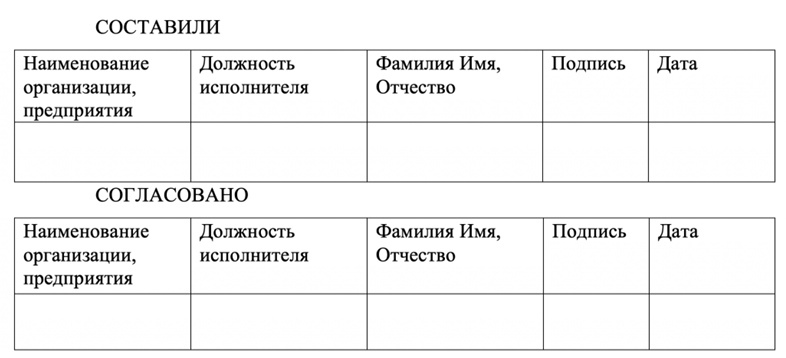
\includegraphics[scale = 0.6]{Рисунки/sostavily.jpg}
\end{document}